\def\lecturenumber{06}
\documentclass[11pt,a4paper]{article}
\usepackage[T1]{fontenc}
\usepackage[utf8]{inputenc}
\usepackage{lmodern}
\usepackage[margin=19mm,top=21mm,bottom=21mm,headheight=15pt]{geometry}
\usepackage{amsmath,amssymb,booktabs,array,graphicx,microtype}
\usepackage[dvipsnames]{xcolor}
\usepackage{enumitem,fancyhdr,listings,tcolorbox}
\usepackage[colorlinks=true,linkcolor=MidnightBlue,urlcolor=MidnightBlue]{hyperref}
\definecolor{courseblue}{HTML}{164B69}
\definecolor{pale}{HTML}{F0F5F7}
\pagestyle{fancy}
\fancyhf{}
\fancyhead[L]{\small\sffamily\color{courseblue}VALIDATED COMPUTING}
\fancyhead[R]{\small\sffamily Lecture \lecturenumber}
\fancyfoot[L]{\footnotesize Expanded lecture notes \textbullet\ October 2026}
\fancyfoot[R]{\footnotesize\thepage\ / 6}
\renewcommand{\headrulewidth}{0.4pt}
\setlength{\parindent}{0pt}
\setlength{\parskip}{5.5pt plus 1pt}
\setlength{\emergencystretch}{1.5em}
\setlist[itemize]{leftmargin=1.5em,itemsep=3pt,topsep=3pt}
\setlist[enumerate]{leftmargin=1.7em,itemsep=5pt,topsep=4pt}
\lstset{language=Python,basicstyle=\small\ttfamily,keywordstyle=\color{courseblue}\bfseries,
 commentstyle=\color{OliveGreen},stringstyle=\color{BrickRed},showstringspaces=false,
 columns=fullflexible,keepspaces=true,frame=single,rulecolor=\color{black!18},
 backgroundcolor=\color{black!2},aboveskip=6pt,belowskip=6pt,breaklines=true,
 xleftmargin=5pt,xrightmargin=5pt,framesep=5pt}
\newcommand{\R}{\mathbb R}
\newcommand{\fl}{\operatorname{fl}}
\newcommand{\abs}[1]{\left|#1\right|}
\newcommand{\heading}[2]{\section*{\color{courseblue}#1}\vspace{-4pt}{\small\sffamily\color{black!65}#2}\par\vspace{3pt}}
\newcommand{\opening}[2]{{\Large\sffamily\bfseries\color{courseblue}Lecture \lecturenumber\quad #1\par}\vspace{5pt}{\small #2}\par}
\newtcolorbox{question}[1]{colback=pale,colframe=courseblue!55,boxrule=0.4pt,
 arc=1mm,left=7pt,right=7pt,top=4pt,bottom=4pt,title={#1},fonttitle=\bfseries\small,
 coltitle=courseblue,colbacktitle=pale}
\newcommand{\reading}[1]{{\footnotesize\textbf{Reading and notebook.} #1\par}}
\hypersetup{pdfauthor={Validated Computing course},pdfsubject={Expanded introductory lecture notes with questions and exercises}}

\hypersetup{pdftitle={Lecture 06: Dependency, range bounds, and subdivision}}
\begin{document}
\opening{Dependency, range bounds, and subdivision}{Prerequisites: Lectures 04--05; elementary derivatives and Python loops.\newline
Goal: explain wide enclosures, improve them without losing coverage, and distinguish a bound from a proof of a root.}
\heading{1. A valid enclosure need not be a sharp range}{0--13 minutes: definitions and a diagnostic example}

For a real function $f$ and an interval $X$ contained in its domain, the
\emph{range} is the set $f(X)=\{f(x):x\in X\}$. An interval evaluator $F$
is an \emph{inclusion function} when
\[
                     f(X)\subseteq F(X).
\]
The left side describes the mathematical problem; the right side is what our
algorithm returns. A continuous function on a closed, bounded interval has a
minimum and a maximum, so its range is itself a closed interval. Computing
those two extrema exactly can nevertheless be difficult.

Replacing each operation in an expression by a valid interval operation gives
a \emph{natural interval extension}. The inclusion proof follows the expression
tree: each intermediate interval contains every intermediate real value.
This proves validity, but it does not prove that every number in the final
interval occurs as a function value. Wider intermediate sets can introduce
combinations of values that no single input can produce.

For example, take $f(x)=x^2+1$ on $X=[-1,1]$. Independent interval multiplication
gives $X\cdot X=[-1,1]$, and hence $X\cdot X+1=[0,2]$. The sharp square operation
instead gives $\operatorname{sqr}(X)+1=[1,2]$, the exact range. Both enclosures
are valid. Only the second immediately proves that $f$ is strictly positive.

\textbf{Reading a certificate.} If $0\notin F(X)$, then $f$ has no zero in $X$.
If $0\in F(X)$, the conclusion is only ``this enclosure did not exclude a
zero.'' Existence requires another argument, such as a sign change combined
with continuity. A nonnegative lower endpoint proves nonnegativity; a
\emph{strictly} positive lower endpoint proves positivity.

\textbf{A useful additional property.} An evaluator is \emph{inclusion isotonic}
if $X\subseteq Y$ implies $F(X)\subseteq F(Y)$. Exact natural interval
extensions have this property wherever all operations are defined. It explains
why restricting the input can help. Validity alone does not imply isotonicity,
and changing the implementation or precision while comparing outputs requires
care: two valid enclosures need not be nested.

\begin{question}{Discuss before calculating}
An implementation returns $[-100,100]$ for a function whose true range is
$[2,3]$. Is it incorrect? Is it useful for excluding a zero? What changes if
the result is $[2.1,3]$? Identify the missing value that makes the latter fail.
\end{question}

Our objective is to preserve inclusion while making the enclosure useful for
a specific question. Small width is helpful, but it is not the definition of
correctness. Even the exact range can be wide when the function varies greatly.

\newpage
\heading{2. One function, three different computations}{13--30 minutes: work through the algebra together}

Consider $f(x)=x(1-x)$ on $X=[0,1]$. The identities
\[
       x-x^2=x(1-x)=\frac14-\left(x-\frac12\right)^2
\]
hold for every real $x$. Their interval evaluations differ because interval
operations retain ranges of intermediate values, not the relations between
those values. Use a sharp square whenever a square is written explicitly.

\begin{center}
\begin{tabular}{lll}
\toprule
Expression & Interval calculation on $[0,1]$ & Enclosure\\
\midrule
$x-x^2$ & $[0,1]-[0,1]$ & $[-1,1]$\\
$x(1-x)$ & $[0,1]\cdot[0,1]$ & $[0,1]$\\
$\frac14-(x-\frac12)^2$ & $\frac14-[0,\frac14]$ & $[0,\frac14]$\\
\bottomrule
\end{tabular}
\end{center}

The last enclosure is the exact range. Indeed, the square is nonnegative,
so $f(x)\leq 1/4$; also $x\geq0$ and $1-x\geq0$, so $f(x)\geq0$.
The values $f(0)=0$ and $f(1/2)=1/4$ attain the bounds. Continuity supplies
every intermediate value. Equivalently, $f'(x)=1-2x$ changes sign at $1/2$.

\textbf{Where does the false upper bound $1$ come from?}
Introduce $y=1-x$. The exact problem maximizes $xy$ along the line segment
$x+y=1$ inside the square $[0,1]^2$. Independent multiplication maximizes
$xy$ over the whole square. It permits $(x,y)=(1,1)$ even though that pair
violates $y=1-x$. The computation solved a larger problem, whose answer is
still an upper bound for the original one.

This loss of information is called the \emph{dependency problem}. It can occur
even with exact rational endpoints: none of the three calculations in the
table uses rounding. Increasing machine precision therefore cannot remove
these particular excess widths. Precision addresses arithmetic rounding;
rewriting an expression addresses which relations the evaluator preserves.

There is no universal rule that the expanded or factored form is best.
The input interval matters. On $[0,1/4]$, the three forms above give, in order,
$[-1/16,1/4]$, $[0,1/4]$, and $[0,3/16]$. The vertex form remains exact here,
but finding a comparable identity for a complicated function may be difficult.
Subdivision offers a systematic alternative that does not require a perfect
symbolic reformulation.

\begin{question}{Board exercise: trace the repeated variable}
In $X-X^2$, which choices of the two occurrences of $x$ produce the interval
lower bound $-1$? Can one real input make both choices at once? Explain why
the bound is valid despite being unattainable.
\end{question}

\textbf{Practical rule.} Before adding precision or splitting hundreds of
intervals, inspect the formula. A sharp square, an exact identity, or an
analytically known sign may save substantial computation. Check the domain
whenever a rewriting introduces division or another restricted operation.

\newpage
\heading{3. Covering an interval gives a proof}{30--46 minutes: the covering argument and two subintervals}

Suppose closed intervals $X_1,\ldots,X_N$ cover the entire input interval:
$X=\bigcup_{i=1}^N X_i$. Each piece must lie in the domain of the evaluator.
If $f(X_i)\subseteq F(X_i)$ for every piece, then
\[
 f(X)=\bigcup_{i=1}^N f(X_i)
       \subseteq\bigcup_{i=1}^N F(X_i)
       \subseteq\operatorname{hull}\{F(X_1),\ldots,F(X_N)\}.
\]
To prove this, take an arbitrary $x\in X$. Coverage puts $x$ in at least one
piece $X_i$. The local inclusion puts $f(x)$ in $F(X_i)$, and therefore in
the hull. Since $x$ was arbitrary, no input is left out. This is the step that
a finite list of point samples cannot supply.

For sorted pieces of $[a,b]$, check the two outer endpoints and check that
successive pieces touch or overlap. Shared endpoints cause no problem.
A small gap does: it is a region about which the local certificates say
nothing. Exact rational split points make these coverage checks transparent.

For $0\leq a\leq b\leq1$, the product expression for our example gives
\[
 F([a,b])=[a,b]\,[1-b,1-a]=[a(1-b),\ b(1-a)].
\]
All factors are nonnegative, which explains the simple endpoint formula.
It is an enclosure, not generally the exact range on the piece. Splitting
$[0,1]$ into $[0,1/2]$ and $[1/2,1]$ gives $[0,1/2]$ on each piece. Their
hull is $[0,1/2]$, an improvement over $[0,1]$ that still contains $[0,1/4]$.

\begin{lstlisting}
from fractions import Fraction

def product_enclosure(left, right):
    assert 0 <= left <= right <= 1
    return left * (1 - right), right * (1 - left)

def uniform_pieces(left, right, count):
    # Inputs left and right are Fractions; count is an integer.
    if count < 1 or left > right:
        raise ValueError("Need ordered endpoints and count >= 1")
    step = (right - left) / count
    pieces = []
    for index in range(count):
        a = left + index * step
        b = left + (index + 1) * step
        pieces.append((a, b))
    return pieces
\end{lstlisting}

These short functions use exact arithmetic. The assertions document the
example's restricted domain; they are not a general interval library.
The same covering argument works with outward-rounded machine intervals,
provided each local evaluation has a valid inclusion guarantee.

\begin{question}{A logical checkpoint}
If every piece has a strictly positive lower bound, what follows globally?
Would the same conclusion follow if all piece midpoints had positive values?
State the extra information supplied by the interval evaluations.
\end{question}

\newpage
\heading{4. Implement the hull and inspect the improvement}{46--62 minutes: readable code and a geometric picture}

A global enclosure uses the smallest local lower endpoint and the largest
local upper endpoint. This combines certificates; averaging endpoints would
not preserve the inclusion argument. The function below assumes a nonempty
list of covering pieces and an evaluator valid on every piece.

\begin{lstlisting}
def enclose_by_pieces(evaluate, pieces):
    left, right = pieces[0]
    lower, upper = evaluate(left, right)
    for left, right in pieces[1:]:
        local_lower, local_upper = evaluate(left, right)
        lower = min(lower, local_lower)
        upper = max(upper, local_upper)
    return lower, upper

for count in [1, 2, 4, 8, 16]:
    pieces = uniform_pieces(Fraction(0), Fraction(1), count)
    lower, upper = enclose_by_pieces(product_enclosure, pieces)
    print(count, str(lower), str(upper))
\end{lstlisting}

The output upper endpoints are $1$, $1/2$, $3/8$, $5/16$, and $9/32$;
all lower endpoints are zero. Each vertical rectangle below encloses every
point of the function graph over its horizontal input piece. The drawn curve
is illustrative: the endpoint arithmetic and coverage establish the bounds.

\begin{center}
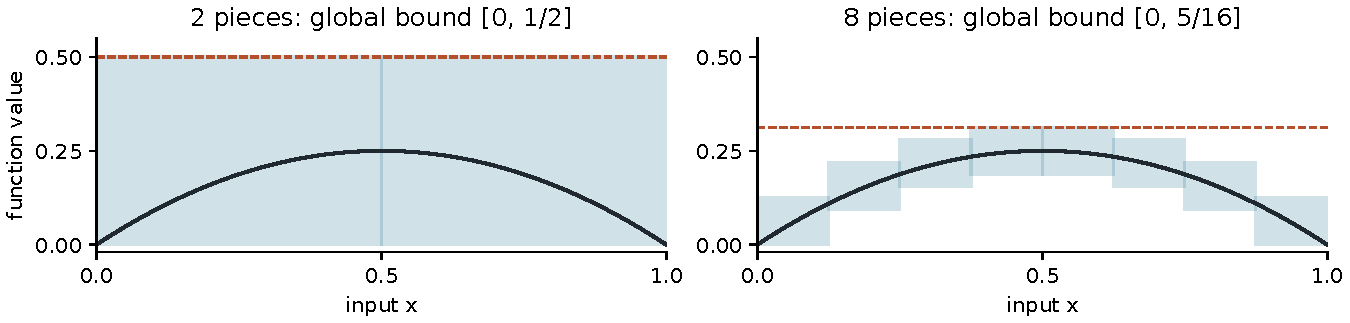
\includegraphics[width=\linewidth]{figures/subdivision_enclosures.pdf}
\end{center}

For an even number $N$ of equal pieces, put $h=1/N$. The upper endpoint on
the piece starting at $a=kh$ is
\[
 (a+h)(1-a)=\frac{(1+h)^2}{4}
                  -\left(a-\frac{1-h}{2}\right)^2.
\]
The nearest allowed starting points to $(1-h)/2$ are $h/2$ away when $N$
is even. Thus the global upper bound is $1/4+h/2=1/4+1/(2N)$.
Halving the mesh halves the excess upper bound in this particular example.
This is a derived result for this evaluator, not a general convergence rate.

\begin{question}{What does refinement converge to?}
Predict the result for $N=32$. Does the width approach zero or $1/4$?
Explain why a nonzero limiting width is compatible with a perfect enclosure.
\end{question}

\newpage
\heading{5. Choose the right remedy for a wide bound}{62--77 minutes: precision, subdivision, and elementary functions}

Width can reflect three different things: variation of the true function,
lost dependence between intermediate quantities, and outward rounding.
Only the last is directly controlled by arithmetic precision. Subdivision
reduces the input variation on each piece and often reduces dependency loss.
The global hull must still include the full variation across all pieces.
For our polynomial, a global width below $1/4$ would be an error.

If a fixed evaluator is inclusion isotonic, each child enclosure is contained
in its parent's enclosure. Replacing a parent by a covering collection of
children then cannot enlarge the global hull. Strict improvement is not
guaranteed. Nor does validity by itself imply that repeated subdivision
converges to the exact range; that requires properties of the evaluator.

\textbf{Stopping honestly.} A maximum number of pieces is a resource limit,
not a proof of a requested accuracy. If the budget is exhausted, report the
current bound and the unmet target. In an adaptive method, unprocessed
pieces must retain valid bounds so that coverage is never silently lost.
Likewise, splitting an interval containing zero does not make $1/x$ defined
at zero. Domain failure requires reformulating the question or reporting it.

For elementary functions, use an implementation with inclusion guarantees.
Evaluating an ordinary \texttt{math.sin} at two endpoints is insufficient:
even exact endpoint values for $[0,\pi]$ would miss the interior maximum $1$.
The course uses Arb through \texttt{python-flint}. Here is a direct example,
independent of the teaching package \texttt{vc}:

\begin{lstlisting}
from flint import arb, ctx, fmpq

with ctx.workprec(100):
    x = arb(0).union(arb(fmpq(1, 2)))
    result = (x.sin() - x * x + 1) * x.cos()
    if not result.is_finite():
        raise ValueError("No finite enclosure was obtained")
    midpoint = result.mid().fmpq()
    radius = result.rad().fmpq()
    lower = midpoint - radius
    assert lower > 0
\end{lstlisting}

The input ball contains $[0,1/2]$. Arb's operations enclose the expression
on that ball; subtracting its exact rational radius from its exact rational
midpoint gives a rigorous lower endpoint. The successful comparison proves
$(\sin x-x^2+1)\cos x>0$ for every $x\in[0,1/2]$. A conversion to a ball
may widen the domain; all operations must be valid on that enlarged input too.

\begin{question}{Explain the scope of the computation}
Which line supplies coverage of the input? Which supplies the sign
certificate? Why would a positive printed midpoint alone be insufficient?
If the assertion failed, would that prove that the function has a zero?
\end{question}

\reading{The elementary-function example accompanies Notebook/Lab 06.
API reference: \href{https://python-flint.readthedocs.io/en/latest/arb.html}{python-flint, real balls (\texttt{arb})}.}

\newpage
\heading{6. Exercises, checks, and a certificate audit}{77--90 minutes: select two exercises; finish the others independently}

\begin{enumerate}
\item \textbf{Formula choice.} On $X=[0,1/4]$, evaluate $X-X^2$,
$X(1-X)$, and $1/4-(X-1/2)^2$ using sharp squares. Verify the three bounds
on page 2. Use monotonicity of $x(1-x)$ on this interval to find its exact
range. Which forms introduce unattainable values, and where?

\item \textbf{Prove positivity.} Let $g(x)=x^2-x+1$ on $[0,1]$.
The natural expanded expression gives $[0,2]$. Explain precisely why that
result does not prove strict positivity. Rewrite the expression to obtain
the exact range and a positive lower bound. Would higher precision alone
improve the exact-arithmetic expanded enclosure?

\item \textbf{The missing piece.} A program checks only $[0,49/100]$ and
$[51/100,1]$ for $q(x)=(x-1/2)^2$. It obtains a strictly positive lower
bound on each piece and declares no roots on $[0,1]$. Find the error and
the missed root. Repair the cover, and predict why the repaired calculation
can no longer certify strict positivity.

\item \textbf{Set a meaningful budget.} For the product evaluator and
equal subdivision of $[0,1]$, use the upper-bound formula for even $N$.
What is the smallest power of two $N$ for which the upper bound exceeds
the true maximum by at most $1/100$? Could any valid subdivision produce
a global enclosure of width at most $1/100$? Distinguish these two targets.

\item \textbf{Validity versus isotonicity (optional).} Let $f(x)=0$ for all
real $x$. Define $F(X)=[-1,1]$ if the width of $X$ is less than $1$, and
$F(X)=[0,0]$ otherwise. Show that $F$ is always an inclusion function.
Use $X=[0,1/2]\subset Y=[0,2]$ to disprove isotonicity. What happens to
the enclosure when $Y$ is split into four equal pieces?
\end{enumerate}

\textbf{Selected checks.} Exercise 1: the bounds are $[-1/16,1/4]$,
$[0,1/4]$, and $[0,3/16]$; the last is the exact range since
$f'(x)=1-2x\geq1/2$ on this input. Exercise 2:
$g(x)=(x-1/2)^2+3/4$ gives $[3/4,1]$. Exercise 3: the missed root is
$1/2$; each checked piece has exact lower bound $1/10000$, but together
they do not cover the input. Adding the middle piece includes a zero value.
Exercise 4: $1/(2N)\leq1/100$ requires $N\geq50$, so the smallest power
of two is $64$. The actual range has width $1/4$, ruling out the second
target. Exercise 5: the parent returns $[0,0]$, while the children's hull
is $[-1,1]$. Both are valid, but subdivision worsened the result.

\begin{question}{Certificate audit: say all the premises}
Complete this claim: ``The function is positive on the whole interval
because\ldots'' Your explanation must identify the exact function and
domain, the covering pieces, a valid local evaluator, and the strict sign
of every local lower bound. State what a failed check leaves undecided.
\end{question}

\textbf{Before the next lecture.} Run the exact-rational subdivision example
and retain the endpoint fractions. Try a different formula on each piece,
keeping coverage fixed. Notebook 06 provides further experiments; Lecture 07
adds derivative information to obtain sharper bounds and faster certificates.

\reading{Tucker, \emph{Validated Numerics}, \S3.1 (pp.~46--54), especially
Examples 3.1.1--3.1.4 and Theorem 3.8. These notes use original derivations;
the numbered notebook and lab provide the executable course companion.}
\end{document}
